% Options for packages loaded elsewhere
\PassOptionsToPackage{unicode}{hyperref}
\PassOptionsToPackage{hyphens}{url}
\PassOptionsToPackage{dvipsnames,svgnames,x11names}{xcolor}
%
\documentclass[
  letterpaper,
  DIV=11,
  numbers=noendperiod]{scrreprt}

\usepackage{amsmath,amssymb}
\usepackage{iftex}
\ifPDFTeX
  \usepackage[T1]{fontenc}
  \usepackage[utf8]{inputenc}
  \usepackage{textcomp} % provide euro and other symbols
\else % if luatex or xetex
  \usepackage{unicode-math}
  \defaultfontfeatures{Scale=MatchLowercase}
  \defaultfontfeatures[\rmfamily]{Ligatures=TeX,Scale=1}
\fi
\usepackage{lmodern}
\ifPDFTeX\else  
    % xetex/luatex font selection
\fi
% Use upquote if available, for straight quotes in verbatim environments
\IfFileExists{upquote.sty}{\usepackage{upquote}}{}
\IfFileExists{microtype.sty}{% use microtype if available
  \usepackage[]{microtype}
  \UseMicrotypeSet[protrusion]{basicmath} % disable protrusion for tt fonts
}{}
\makeatletter
\@ifundefined{KOMAClassName}{% if non-KOMA class
  \IfFileExists{parskip.sty}{%
    \usepackage{parskip}
  }{% else
    \setlength{\parindent}{0pt}
    \setlength{\parskip}{6pt plus 2pt minus 1pt}}
}{% if KOMA class
  \KOMAoptions{parskip=half}}
\makeatother
\usepackage{xcolor}
\usepackage[top=3cm,left=3cm,right=2cm,bottom=2cm]{geometry}
\setlength{\emergencystretch}{3em} % prevent overfull lines
\setcounter{secnumdepth}{5}
% Make \paragraph and \subparagraph free-standing
\ifx\paragraph\undefined\else
  \let\oldparagraph\paragraph
  \renewcommand{\paragraph}[1]{\oldparagraph{#1}\mbox{}}
\fi
\ifx\subparagraph\undefined\else
  \let\oldsubparagraph\subparagraph
  \renewcommand{\subparagraph}[1]{\oldsubparagraph{#1}\mbox{}}
\fi


\providecommand{\tightlist}{%
  \setlength{\itemsep}{0pt}\setlength{\parskip}{0pt}}\usepackage{longtable,booktabs,array}
\usepackage{calc} % for calculating minipage widths
% Correct order of tables after \paragraph or \subparagraph
\usepackage{etoolbox}
\makeatletter
\patchcmd\longtable{\par}{\if@noskipsec\mbox{}\fi\par}{}{}
\makeatother
% Allow footnotes in longtable head/foot
\IfFileExists{footnotehyper.sty}{\usepackage{footnotehyper}}{\usepackage{footnote}}
\makesavenoteenv{longtable}
\usepackage{graphicx}
\makeatletter
\def\maxwidth{\ifdim\Gin@nat@width>\linewidth\linewidth\else\Gin@nat@width\fi}
\def\maxheight{\ifdim\Gin@nat@height>\textheight\textheight\else\Gin@nat@height\fi}
\makeatother
% Scale images if necessary, so that they will not overflow the page
% margins by default, and it is still possible to overwrite the defaults
% using explicit options in \includegraphics[width, height, ...]{}
\setkeys{Gin}{width=\maxwidth,height=\maxheight,keepaspectratio}
% Set default figure placement to htbp
\makeatletter
\def\fps@figure{htbp}
\makeatother

\usepackage{booktabs}
\usepackage{longtable}
\usepackage{array}
\usepackage{multirow}
\usepackage{wrapfig}
\usepackage{float}
\usepackage{colortbl}
\usepackage{pdflscape}
\usepackage{tabu}
\usepackage{threeparttable}
\usepackage{threeparttablex}
\usepackage[normalem]{ulem}
\usepackage{makecell}
\usepackage{xcolor}
\KOMAoption{captions}{tableheading,figureheading}
\makeatletter
\@ifpackageloaded{caption}{}{\usepackage{caption}}
\AtBeginDocument{%
\ifdefined\contentsname
  \renewcommand*\contentsname{Índice}
\else
  \newcommand\contentsname{Índice}
\fi
\ifdefined\listfigurename
  \renewcommand*\listfigurename{Lista de Figuras}
\else
  \newcommand\listfigurename{Lista de Figuras}
\fi
\ifdefined\listtablename
  \renewcommand*\listtablename{Lista de Tabelas}
\else
  \newcommand\listtablename{Lista de Tabelas}
\fi
\ifdefined\figurename
  \renewcommand*\figurename{Figura}
\else
  \newcommand\figurename{Figura}
\fi
\ifdefined\tablename
  \renewcommand*\tablename{Tabela}
\else
  \newcommand\tablename{Tabela}
\fi
}
\@ifpackageloaded{float}{}{\usepackage{float}}
\floatstyle{ruled}
\@ifundefined{c@chapter}{\newfloat{codelisting}{h}{lop}}{\newfloat{codelisting}{h}{lop}[chapter]}
\floatname{codelisting}{Listagem}
\newcommand*\listoflistings{\listof{codelisting}{Lista de Listagens}}
\makeatother
\makeatletter
\makeatother
\makeatletter
\@ifpackageloaded{caption}{}{\usepackage{caption}}
\@ifpackageloaded{subcaption}{}{\usepackage{subcaption}}
\makeatother
\ifLuaTeX
\usepackage[bidi=basic]{babel}
\else
\usepackage[bidi=default]{babel}
\fi
\babelprovide[main,import]{portuguese}
% get rid of language-specific shorthands (see #6817):
\let\LanguageShortHands\languageshorthands
\def\languageshorthands#1{}
\ifLuaTeX
  \usepackage{selnolig}  % disable illegal ligatures
\fi
\usepackage{bookmark}

\IfFileExists{xurl.sty}{\usepackage{xurl}}{} % add URL line breaks if available
\urlstyle{same} % disable monospaced font for URLs
\hypersetup{
  pdftitle={Analise de sobrevivência},
  pdfauthor={Eliana, Luanna, Barbara, Maria Cecília, Sofia, Victor},
  pdflang={pt},
  colorlinks=true,
  linkcolor={blue},
  filecolor={Maroon},
  citecolor={Blue},
  urlcolor={Blue},
  pdfcreator={LaTeX via pandoc}}

\title{Analise de sobrevivência}
\usepackage{etoolbox}
\makeatletter
\providecommand{\subtitle}[1]{% add subtitle to \maketitle
  \apptocmd{\@title}{\par {\large #1 \par}}{}{}
}
\makeatother
\subtitle{Tempo até a ocorrência da tuberculose}
\author{Eliana, Luanna, Barbara, Maria Cecília, Sofia, Victor}
\date{03/02/2025}

\begin{document}
\maketitle

\renewcommand*\contentsname{Índice}
{
\hypersetup{linkcolor=}
\setcounter{tocdepth}{2}
\tableofcontents
}
\chapter{Introdução}\label{introduuxe7uxe3o}

Os dados utilizados neste projeto referem-se a um estudo sobre o tempo
até a ocorrência de doenças oportunistas em uma coorte de pacientes HIV
positivos atendidos em um Hospital Universitário. As variáveis foram
obtidas a partir de prontuários clínicos. Para cada paciente,
registrou-se o tempo até a ocorrência de algumas doenças ou
sintomatologias caracteristicamente relacionadas à imunodepressão, como
candidíase, tuberculose, sinais hematológicos, herpes zoster, pneumonia
por Pneumocistis.

O banco de dados é composto por 11 variáveis: nove covariáveis (oito
categóricas e uma numérica), o tempo de acompanhamento e uma variável
indicadora de ocorrência de tuberculose. No estudo, o tempo até a
ocorrência da tuberculose foi registrado como variável resposta, com
censura em casos onde as pacientes não foram acompanhadas até o
surgimento da doença (Ver Tabela~\ref{tbl-tabela}).

\begin{longtable}[]{@{}
  >{\raggedright\arraybackslash}p{(\columnwidth - 2\tabcolsep) * \real{0.1773}}
  >{\raggedright\arraybackslash}p{(\columnwidth - 2\tabcolsep) * \real{0.8227}}@{}}

\caption{\label{tbl-tabela}Descrição das variáveis utilizadas no estudo
sobre tuberculose}

\tabularnewline

\toprule\noalign{}
\begin{minipage}[b]{\linewidth}\raggedright
Variável
\end{minipage} & \begin{minipage}[b]{\linewidth}\raggedright
Descrição
\end{minipage} \\
\midrule\noalign{}
\endhead
\bottomrule\noalign{}
\endlastfoot
Sexo & 1 - Masculino, 2 - Feminino. \\
Escolaridade & 0 - Sem escolaridade, 1 - Até quatro anos de estudo, 2 -
Ensino fundamental, 3 - Ensino médio, 4 - Ensino superior. \\
Idade & Idade em anos na entrada do estudo. \\
Uso de drogas injetáveis & 0 - Não, 1 - Sim. \\
Status da doença & 0 - Censura, 1 - Ocorrência da doença. \\
Tempo até a ocorrência & Tempo até a ocorrência da doença
Tuberculose. \\
Candidíase & 0 - Não, 1 - Sim. \\
Sinais hematológicos & 0 - Não, 1 - Sim. \\
Herpes zoster & 0 - Não, 1 - Sim. \\
Pneumonia & 0 - Não, 1 - Sim. \\
Tuberculose & 0 - Não, 1 - Sim. \\

\end{longtable}

\chapter{Metodologia}\label{metodologia}

Primeiramente, foi realizada uma análise descritiva das variáveis em
estudo. Na análise de sobrevivência, essa etapa consiste em utilizar
métodos não-paramétricos. Quase todas as covariáveis são dicotômicas, e,
portanto, foi possível construir as estimativas de Kaplan-Meier para
comparar as duas categorias. Isso foi feito para as 8 covariáveis
categóricas, e também foi testada a hipótese de igualdade das duas
curvas utilizando os testes de Wilcoxon e log-rank. Além disso, foi
analisado se essas covariáveis atendem à suposição de riscos
proporcionais.

A variável ``idade'' foi analisada utilizando o modelo de Cox para
verificar a presença de risco proporcional. Ela também foi estratificada
para análise de diferentes faixas etárias.

A próxima etapa da análise consistiu em modelar separadamente cada uma
das covariáveis com a variável resposta. O objetivo dessa etapa foi
selecionar as variáveis explicativas (covariáveis) que devem prosseguir
para a modelagem. O critério utilizado neste trabalho foi manter as
variáveis que apresentaram valores de p inferiores a 0,25 em pelo menos
um dos testes de Wilcoxon e log-rank na comparação das curvas de
sobrevivência.

No modelo de Cox, as variáveis incluídas no modelo inicial foram aquelas
que apresentaram significância estatística no teste de Wilcoxon ou
log-rank, além de atenderem ao pressuposto de riscos proporcionais. Após
essa seleção inicial, foi realizado um ajuste passo a passo, no qual a
variável com o maior p-valor foi removida iterativamente, até que o
modelo final contivesse apenas variáveis estatisticamente
significativas. Esse processo garantiu um modelo mais parcimonioso e
robusto, mantendo apenas os preditores mais relevantes para a análise da
sobrevivência.

No modelo paramétrico, foi realizado um teste de comparação entre os
modelos de gama generalizada, lognormal, Weibull e exponencial para
escolher o melhor modelo que se ajustasse aos dados. Após essa análise,
foi utilizado o método de backward selection para escolher o modelo
final com as variáveis que mais explicam o tempo até a ocorrência da
tuberculose.

Antes de proceder à interpretação das estimativas dos parâmetros do
modelo ajustado, foram analisados os resíduos para confirmar a adequação
do modelo final escolhido, tanto para o modelo paramétrico quanto para o
semi-paramétrico.

\chapter{Resultados}\label{resultados}

\section{Analise Descritiva e
Exploratória}\label{analise-descritiva-e-exploratuxf3ria}

\begin{figure}

\caption{\label{fig-fig1}Curva de Kaplan-Meier para tuberculose}

\centering{

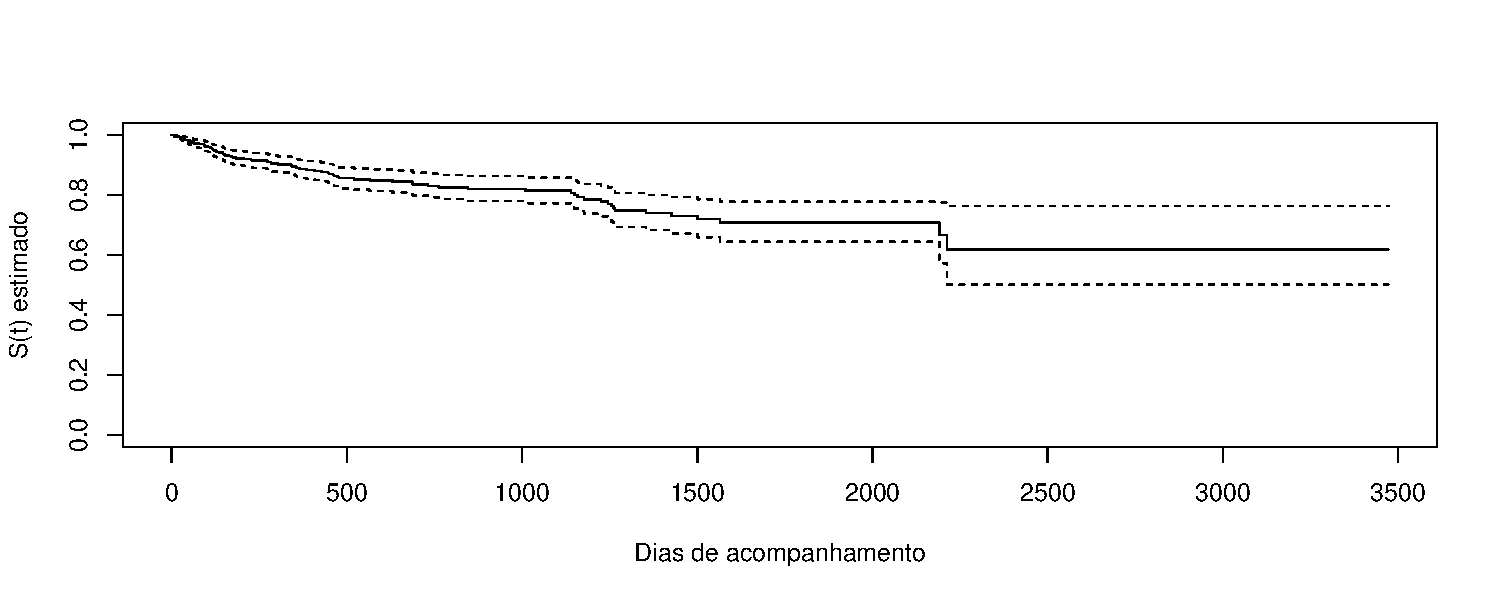
\includegraphics{hj_files/figure-pdf/fig-fig1-1.pdf}

}

\end{figure}%

O gráfico mostra a evolução da probabilidade de não desenvolver
tuberculose ao longo do tempo ( Ver Figura~\ref{fig-fig1}). Com o tempo,
a probabilidade de''sobreviver'' (ou seja, de não desenvolver
tuberculose) diminui à medida que mais indivíduos são diagnosticados com
a doença. Esse gráfico ajuda a identificar em que momento os casos de
tuberculose se acumulam mais rapidamente ou se há períodos de maior
risco.

\begin{figure}

\caption{\label{fig-fig2}Curvas de Kaplan-Meier para sexo}

\centering{

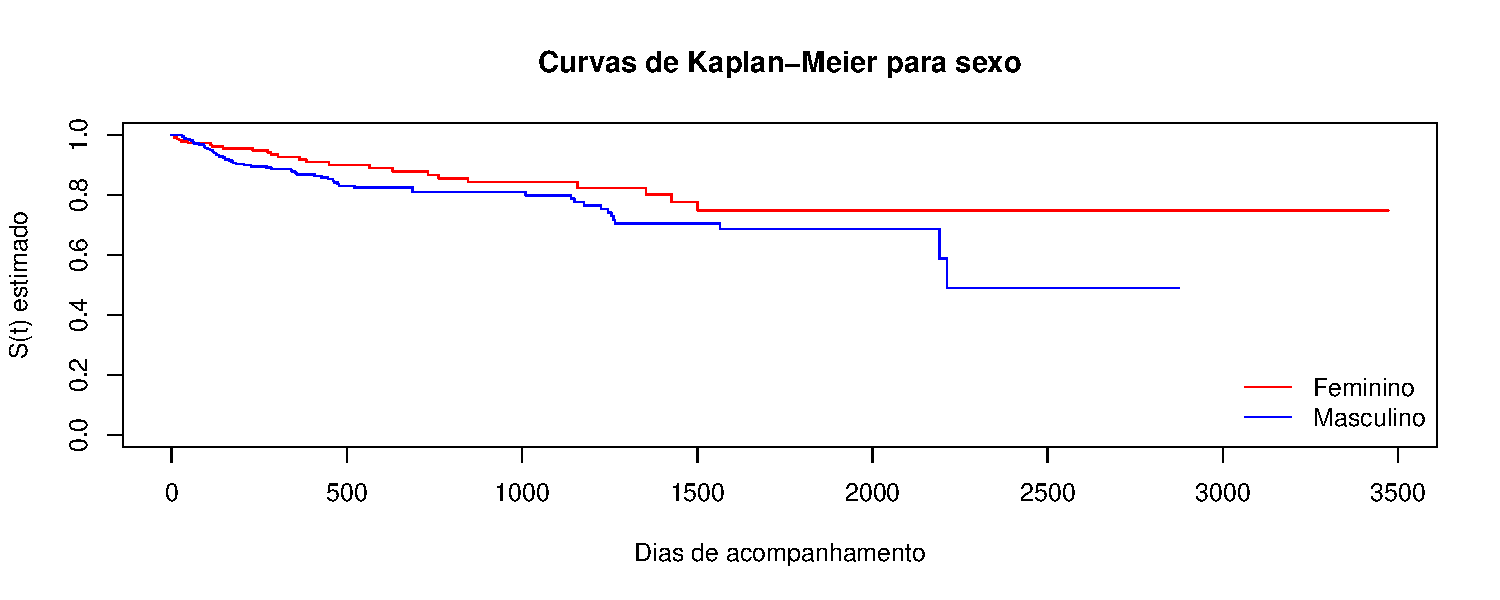
\includegraphics{hj_files/figure-pdf/fig-fig2-1.pdf}

}

\end{figure}%

A curva de Kaplan-Meier para o sexo mostra a probabilidade de não
desenvolver tuberculose ao longo do tempo, separada entre homens e
mulheres ( Ver Figura~\ref{fig-fig2}). No gráfico, a curva das mulheres
(vermelha) está acima da curva dos homens (azul), indicando que as
mulheres têm uma maior probabilidade de não desenvolver a doença ao
longo do tempo, ou seja, elas permanecem ``saudáveis'' por mais tempo.
Em contraste, os homens têm um risco maior, com a curva masculina caindo
mais rapidamente, sugerindo que a probabilidade de desenvolver
tuberculose é maior entre eles. Esse padrão pode indicar que o sexo
masculino está associado a um risco elevado de tuberculose, enquanto o
sexo feminino seria um fator de proteção. Para a variável sex, o p-valor
= 0.86, indicando que não há evidência de violação da suposição de
proporcionalidade dos riscos.

\begin{figure}

\caption{\label{fig-fig3}Curvas de Kaplan-Meier para escolariedade}

\centering{

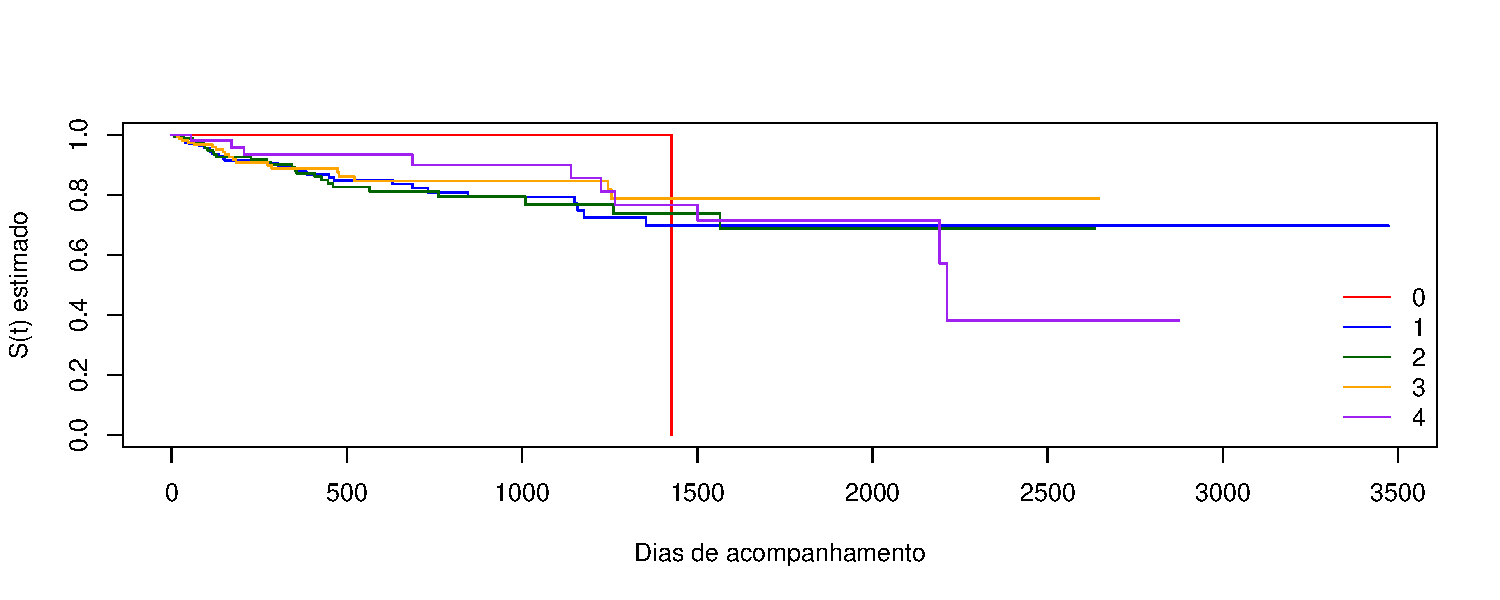
\includegraphics{hj_files/figure-pdf/fig-fig3-1.pdf}

}

\end{figure}%

O gráfico de Kaplan-Meier mostra as curvas de sobrevivência
estratificadas por níveis de escolaridade ( Ver Figura~\ref{fig-fig3}),
indicando que grupos com maior escolaridade (principalmente o ensino
superior) tendem a ter maior sobrevida, enquanto o grupo sem
escolaridade apresenta uma curva mais baixa, embora com poucas
observações (7), o que pode limitar a confiabilidade dessa estimativa.
As curvas não violam o pressuposto de riscos proporcionais, permitindo o
uso adequado do modelo de Cox para análise mais detalhada.Para a
variável escolaridade, o p-valor = 0.31, indicando que não há evidência
de violação da suposição de proporcionalidade dos riscos.

\begin{figure}

\caption{\label{fig-fig4}Curvas de Kaplan-Meier para Uso de drogas
injetáveis}

\centering{

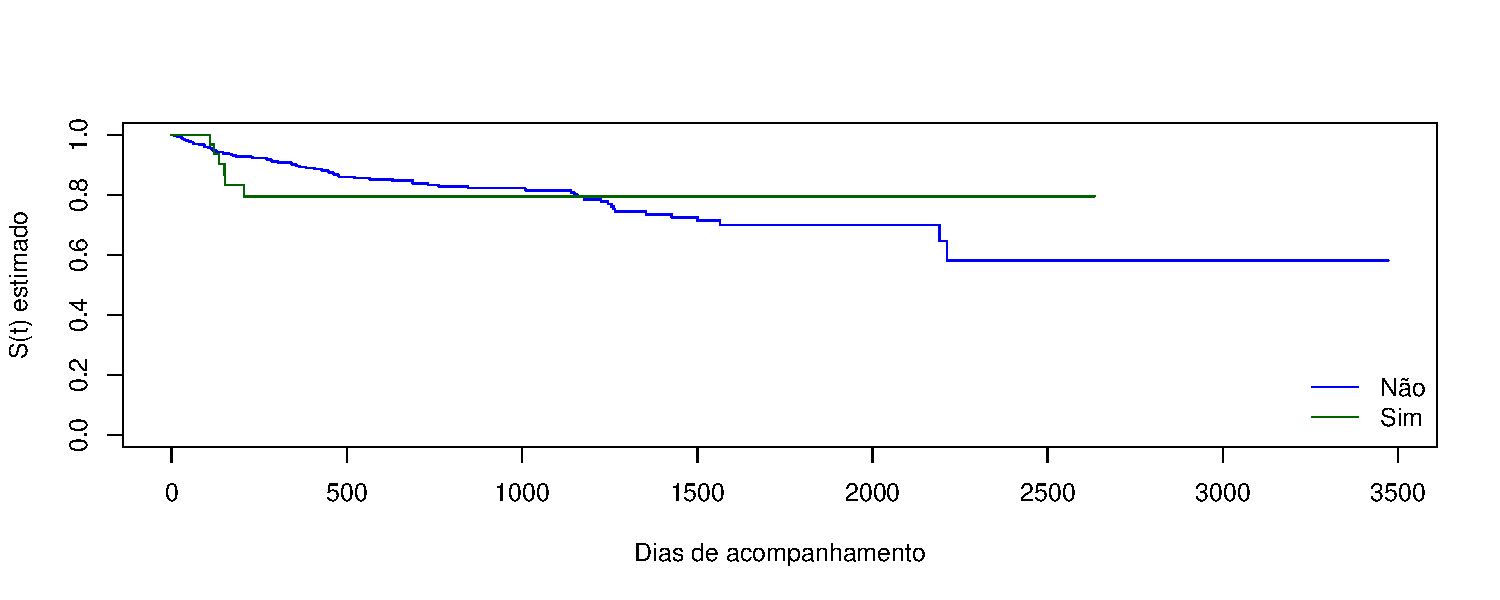
\includegraphics{hj_files/figure-pdf/fig-fig4-1.pdf}

}

\end{figure}%

O gráfico de Kaplan-Meier apresenta as curvas de sobrevivência para
indivíduos que usam ou não drogas injetáveis ( Ver
Figura~\ref{fig-fig4}). Observa-se que o grupo que não usa drogas
injetáveis (linha azul) possui uma probabilidade de sobrevivência maior
ao longo do tempo em comparação ao grupo que usa (linha verde), até o
dia 1100, aproximadamente. Depois disso, as curvas são invertidas. A
curva daqueles que usam drogas injetáveis se estabiliza perto do dia
200, uma vez que, entre aqueles que são usuários, o último que teve
ocorrência da doença foi no dia 206. Apesar disso, as curvas não violam
o pressuposto de riscos proporcionais, permitindo o uso do modelo de Cox
para análise adicional. Para a variável escolaridade, o p-valor = 0.092,
indicando que não há evidência de violação da suposição de
proporcionalidade dos riscos.

\begin{figure}

\caption{\label{fig-fig5}Curvas de Kaplan-Meier para sexualidade}

\centering{

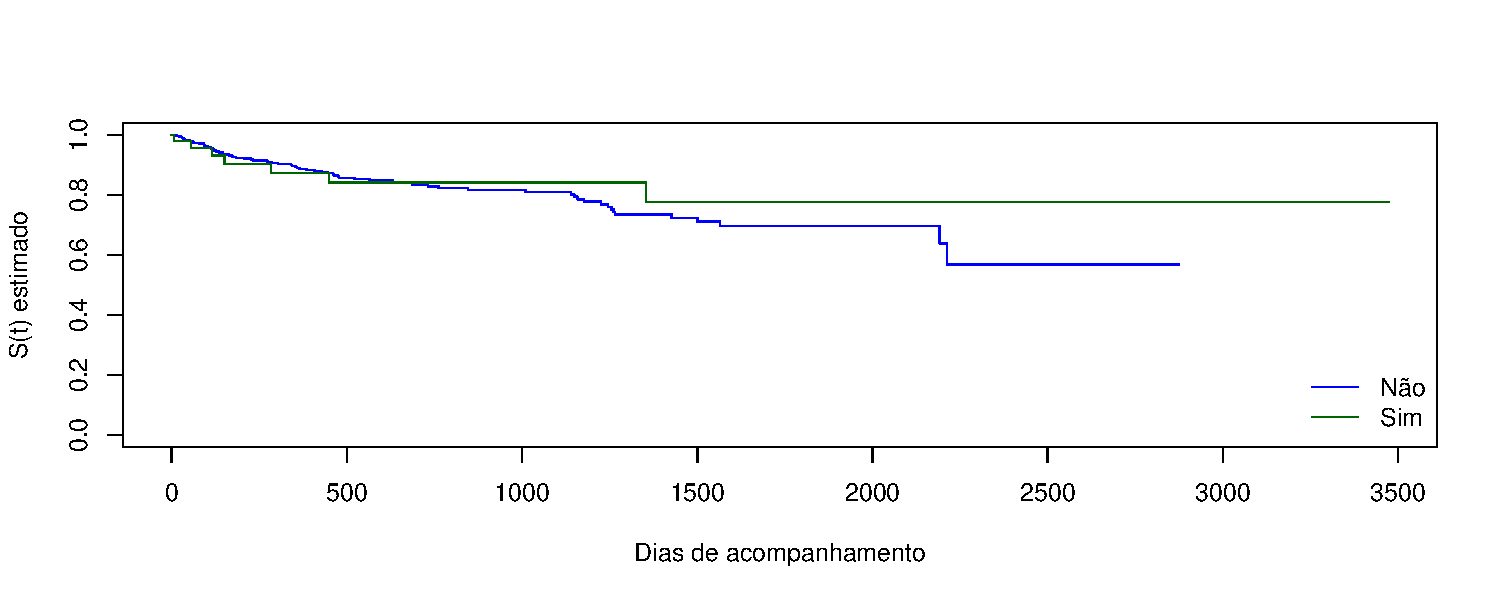
\includegraphics{hj_files/figure-pdf/fig-fig5-1.pdf}

}

\end{figure}%

O gráfico de Kaplan-Meier apresenta as curvas de sobrevivência para
indivíduos de acordo com a orientação sexual ( Ver
Figura~\ref{fig-fig5}).. Observa-se que o grupo de heterossexuais (linha
azul) possui uma probabilidade de sobrevivência parecida ao longo do
tempo em comparação aos não heterossexuais (linha verde), até o dia 600,
aproximadamente. Depois disso, as curvas são invertidas. Para a variável
sexualidade, o p-valor = 0.16, indicando que não há evidência de
violação da suposição de proporcionalidade dos riscos.

\begin{figure}

\caption{\label{fig-fig6}Curvas de Kaplan-Meier para Candidíase}

\centering{

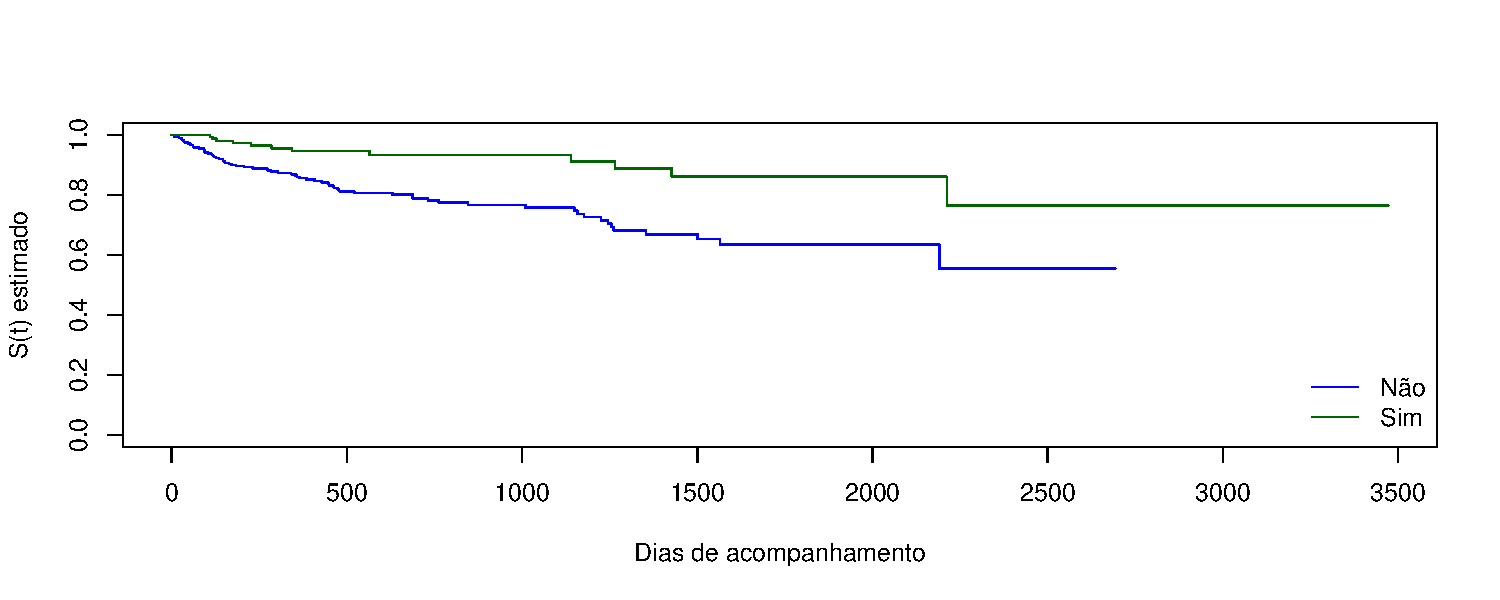
\includegraphics{hj_files/figure-pdf/fig-fig6-1.pdf}

}

\end{figure}%

A curva daqueles com candidíase (verde) está acima daqueles sem (azul),
indicando que pessoas com candidíase têm uma maior probabilidade de não
desenvolver a doença ao longo do tempo, ou seja, elas permanecem
``saudáveis'' por mais tempo ( Ver Figura~\ref{fig-fig6}). Aqueles sem
candidíase têm um risco maior, com a curva caindo mais rapidamente,
sugerindo que a probabilidade de desenvolver tuberculose é maior entre
eles. O pressuposto de risco proporcional é atendido. Para a variável
Candidíase o p-valor = 0.25, indicando que não há evidência de violação
da suposição de proporcionalidade dos riscos.

\begin{figure}

\caption{\label{fig-fig7}Curvas de Kaplan-Meier para Sinais
hematológicos}

\centering{

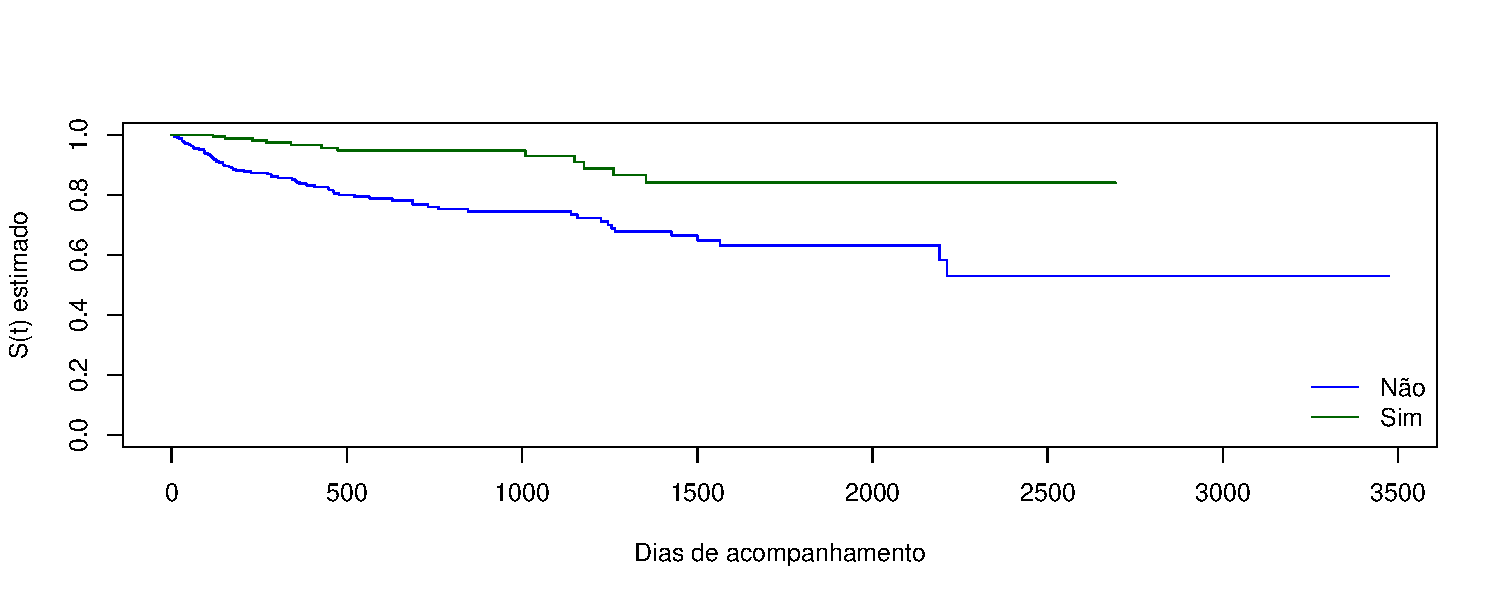
\includegraphics{hj_files/figure-pdf/fig-fig7-1.pdf}

}

\end{figure}%

A curva daqueles com sinais hematológicos (verde) está acima daqueles
sem (azul), indicando que pessoas com sinais hematológicos têm uma maior
probabilidade de não desenvolver a doença ao longo do tempo, ou seja,
elas permanecem ``saudáveis'' por mais tempo ( Ver
Figura~\ref{fig-fig7}). Aqueles sem sinais hematológicos têm um risco
maior, com a curva caindo mais rapidamente, sugerindo que a
probabilidade de desenvolver tuberculose é maior entre eles.Para a
variável Sinais hematológicos, o p-valor = 0.045, indicando que há
evidência de violação da suposição de proporcionalidade dos riscos.

\begin{figure}

\caption{\label{fig-fig8}Curvas de Kaplan-Meier para herpes}

\centering{

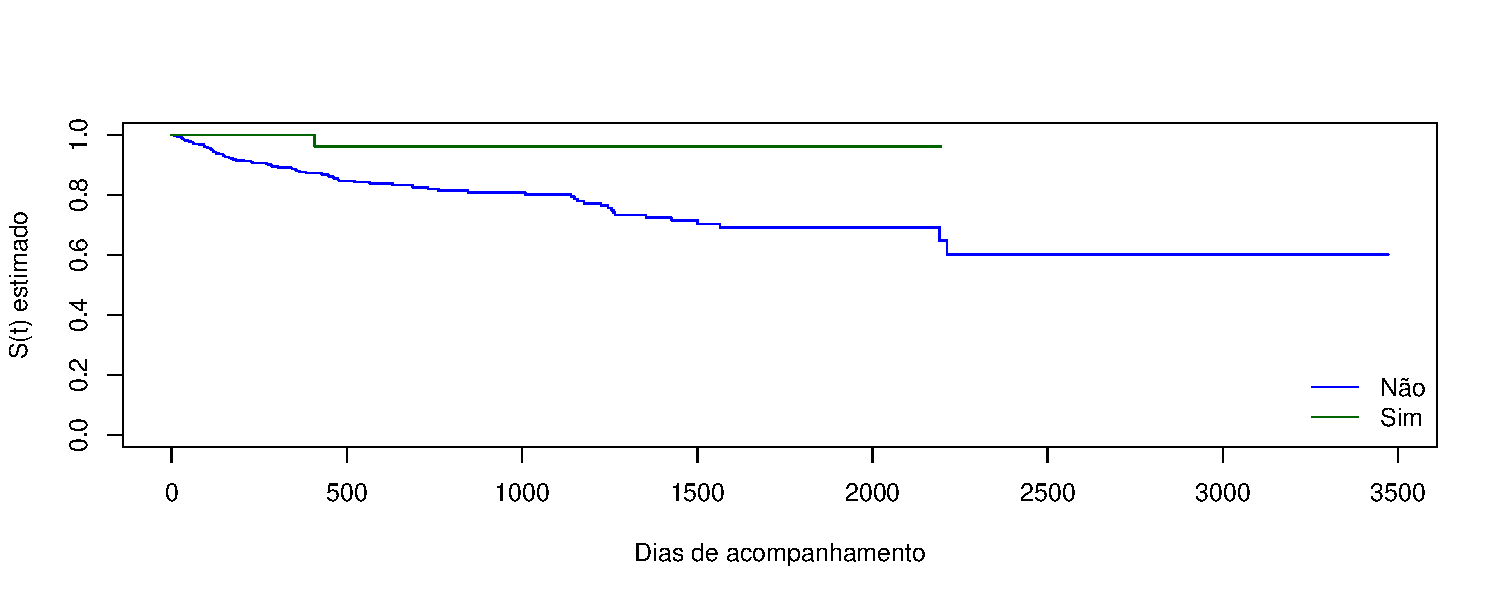
\includegraphics{hj_files/figure-pdf/fig-fig8-1.pdf}

}

\end{figure}%

A curva daqueles com herpes (verde) está acima daqueles sem (azul),
indicando que pessoas com herpes têm uma maior probabilidade de não
desenvolver a doença ao longo do tempo, ou seja, elas permanecem
``saudáveis'' por mais tempo ( Ver Figura~\ref{fig-fig8}). Aqueles sem
herpes têm um risco maior, com a curva caindo mais rapidamente,
sugerindo que a probabilidade de desenvolver tuberculose é maior entre
eles. Para a variável herpes, o p-valor = 0.72, indicando que não há
evidência de violação da suposição de proporcionalidade dos riscos.

\begin{figure}

\caption{\label{fig-fig9}Curvas de Kaplan-Meier para Pneumonia}

\centering{

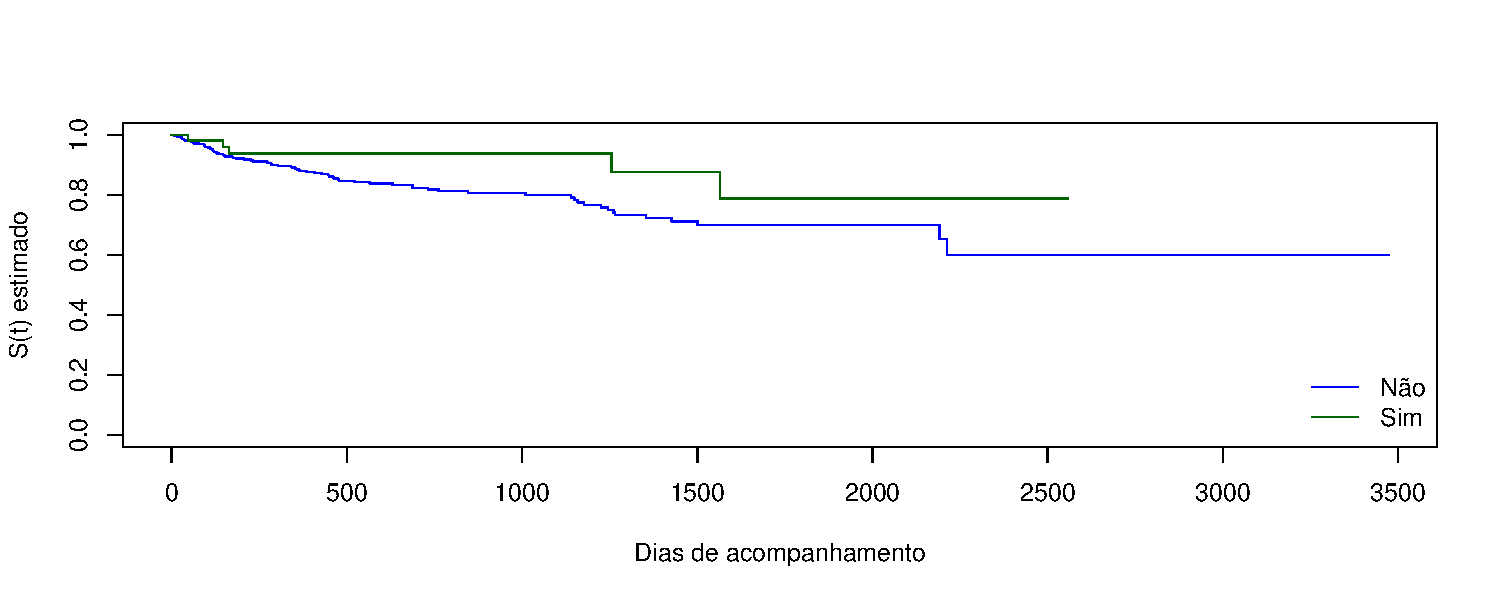
\includegraphics{hj_files/figure-pdf/fig-fig9-1.pdf}

}

\end{figure}%

A curva daqueles com pneumonia (verde) está acima daqueles sem (azul),
indicando que pessoas com pneumonia têm uma maior probabilidade de não
desenvolver a doença ao longo do tempo, ou seja, elas permanecem
``saudáveis'' por mais tempo ( Ver Figura~\ref{fig-fig9}). Aqueles sem
pneumonia têm um risco maior, com a curva caindo mais rapidamente,
sugerindo que a probabilidade de desenvolver tuberculose é maior entre
eles. Para a variável pneumonia, o p-valor = 0.66, indicando que não há
evidência de violação da suposição de proporcionalidade dos riscos.

O teste cox.zph foi aplicado para verificar se o pressuposto de riscos
proporcionais é atendido no modelo de Cox para a variável idade. A
violação desse pressuposto indica que o efeito da idade sobre o risco de
desenvolver tuberculose não é constante ao longo do tempo. Ou seja, a
relação entre a idade e o risco de tuberculose varia durante o período
de acompanhamento, o que invalida o modelo de Cox simples. Isso sugere
que, para modelar adequadamente os dados, pode ser necessário ajustar o
modelo por meio de estratificação.

\begin{figure}

\caption{\label{fig-fig11}Curvas de Kaplan-Meier para idade
estratificada}

\centering{

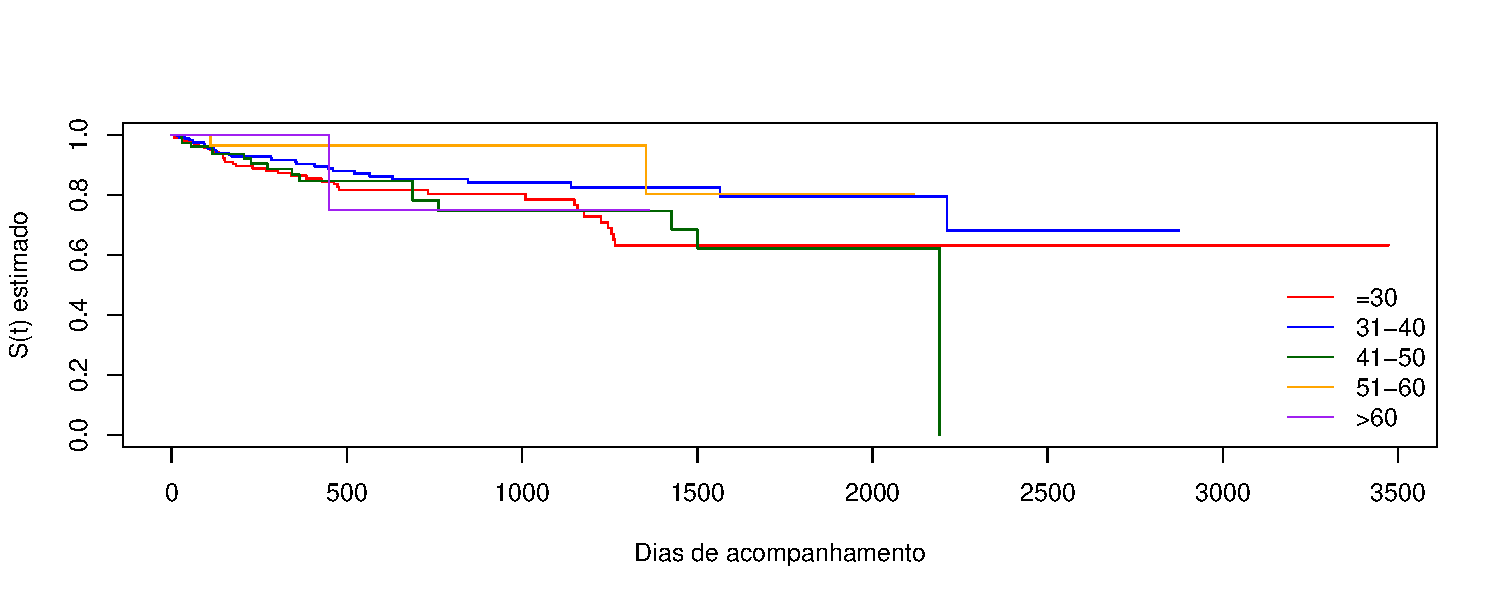
\includegraphics{hj_files/figure-pdf/fig-fig11-1.pdf}

}

\end{figure}%

O gráfico de Kaplan-Meier ilustra as curvas de sobrevivência para
diferentes faixas etárias (≤30, 31--40, 41--50, 51--60, \textgreater60
anos) ao longo do tempo de acompanhamento ( Ver Figura~\ref{fig-fig11}).
Observa-se que o grupo mais jovem (≤30 anos, linha vermelha) apresenta a
maior redução na probabilidade de sobrevivência nos primeiros 1.000
dias, indicando um risco mais elevado de desfecho adverso nesse período.
Por outro lado, os grupos mais velhos (\textgreater60 anos, linha roxa,
e 51--60 anos, linha verde) apresentam melhores probabilidades de
sobrevivência, com declínios mais graduais ao longo do tempo. Essa
tendência sugere que a idade está associada ao risco de desfecho, com
indivíduos mais jovens apresentando maior vulnerabilidade inicial.
Apesar disso, as curvas não violam o pressuposto de riscos
proporcionais,p= 0.55, permitindo o uso do modelo de Cox para análise
adicional.



\end{document}
